%ju 31-Dez-22 Datenkommunikation-im-Frg.tex
\section{Bordelektrik}\label{bordelektrik}

\subsection{Bordnetz}\label{bordnetz}

\begin{figure}[!ht]% hier: !ht
\centering
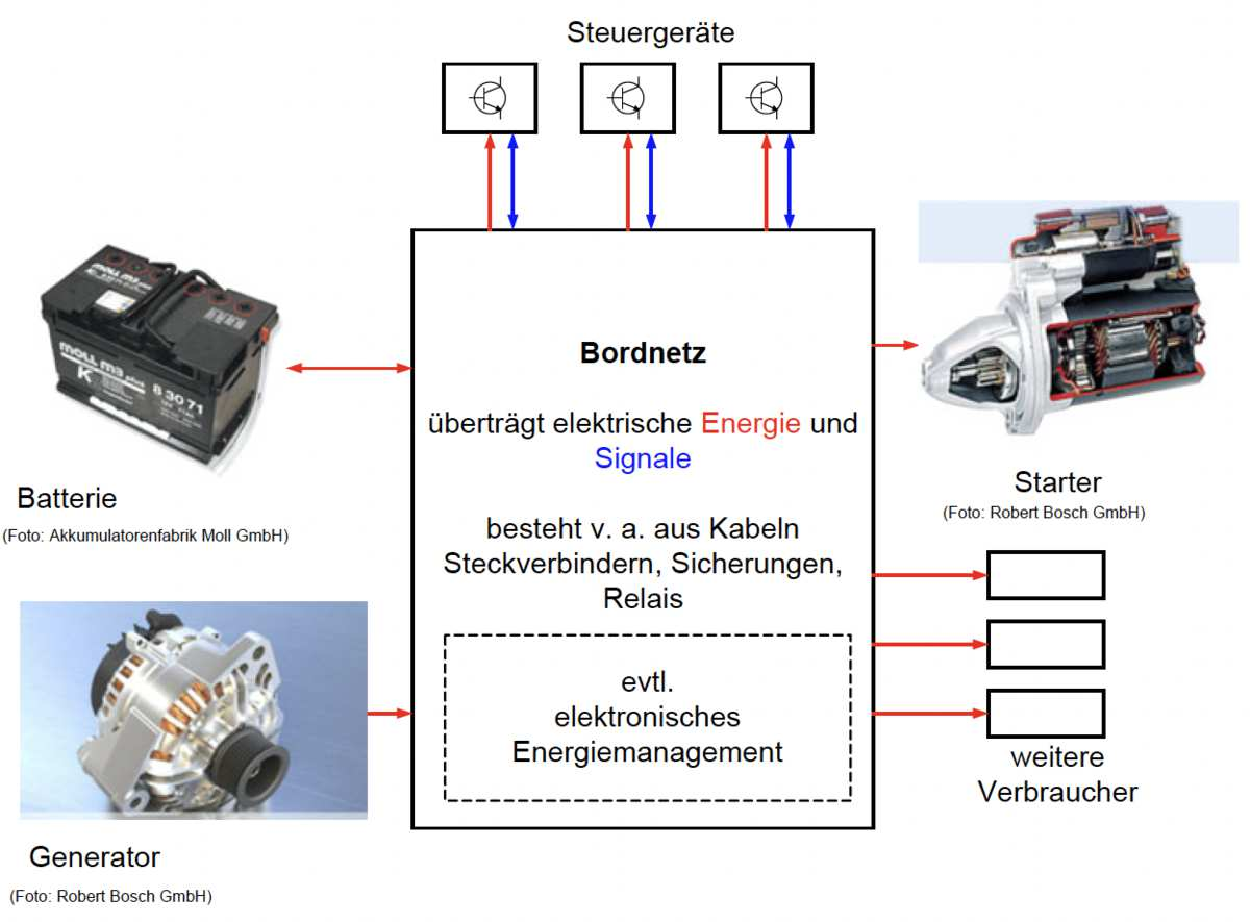
\includegraphics[width=0.7\textwidth]{images/CAN/CAN-1.pdf}
\caption{Überblick über das Bordnetz. (Bild: Kai Borgeest)}
%\label{fig:}%% anpassen
\end{figure}

\textbf{Leitungen}

Um eine unzulässige Erhitzung von Kabeln im normalen Betrieb zu
verhindern, darf die zulässige Stromdichte S nicht überschritten werden.

$S = \frac{I}{A}$ (Stromdichte S, Strom I und dem Leitungsquerschnitt
A)

\textbf{grobe Richtwerte für zulässige Stromdichten}

\begin{itemize}
\item
  Dauerbetrieb $5~A/mm^2$
\item
  kurzzeitige Stromspitzen $10~A/mm^2$
\end{itemize}

Wird die zulässige Stromdichte überschritten, führt die Verlustleistung
$P_V$ in der Leitung zu einer Überhitzung und damit zum Schmelzen, zur
Zersetzung oder zum Brennen des Isoliermaterials oder angrenzender
Strukturen, bei erheblicher Überlast auch zum Schmelzen des Leiters.

\textbf{Verlustleistung beim Strom I}

$P_v = I^2 \cdot R \quad R = \frac{\rho \cdot l}{A}$ (Kupferleitung
$0,0185~\Omega mm^2/m$)

$I = \frac{P}{U}$

\newpage

\textbf{elektrischer Verbraucher 12-V-Bordnetz}

\begin{table}[!ht]% hier: !ht 
\centering 
	\caption{}% \label{tab:}%% anpassen 
\begin{tabular}{@{}lll@{}}
\hline
\textbf{Verbraucher} & \textbf{Leistungsaufnahme P} & \textbf{Strom
I} \\
\hline
Elektro-Kraftstoffpumpe & 250 W & 21 \\
Heckscheibenheizung & 200 W & 17 \\
Innengebläse & 120 W & 10 \\
Kühlerventilator & 120 W & 10 \\
Abblendlicht & 110 W & 9,2 \\
Scheibenwischer & 50 W & 4,2 \\
Bremslicht & 42 W & 3,5 \\
Kennzeichenleuchte & 30 W & 2,5 \\
Standlicht & 8 W & 0,7 \\
\hline
\end{tabular} 
\end{table}

\textbf{Elektro- und Hybridfahrzeugen}

Ab 60 V hat sich der Begriff Hochvoltkabel durchgesetzt. Hochvoltkabel
haben eine geerdete Abschirmung, sind mechanisch besonders stabil und
durch ihre orange Farbgebung auffällig gekennzeichnet.

Hochvoltkomponenten werden durch eine ringförmige Niederspannungsleitung
verbunden (HVIL, High Voltage Interlock Loop), die auf Unterbrechungen
überwacht wird. Wird eine Unterbrechung durch Trennung einer Leitung
oder Öffnung eines Gehäuses erkannt, führt dies zur Abschaltung des
Hochvoltsystems.

\textbf{Klemmenbezeichnungen} (Auswahl)

\begin{table}[!ht]% hier: !ht 
\centering 
	\caption{}% \label{tab:}%% anpassen 
\begin{tabular}{@{}ll@{}}
\hline
\textbf{Nr.} & \textbf{Bezeichnung} \\
\hline
1 & Zündspule (gemeinsame Klemme) \\
4 & Zündspule (Hochspannungsausgang) \\
15 & Positive Batteriespannung, über Schlüsselschalter \\
30 & Positive Batteriespannung \\
31 & Negative Batteriespannung \\
50 & Anlasser (geschaltete Klemme) \\
54 -- 58 & Beleuchtung \\
81 -- 88 & Schalter und Relais \\
B+ & Positive Generatorklemme zur Batterie \\
B & Negative Generatorklemme zur Batterie \\
D+ & Positive Klemme an Generator und Regler für Regelung und Leuchte \\
D & Negative Klemme an Generator und Regler für Regelung und Leuchte \\
DF & >>Dynamo Feld<<, Klemme an Generator und Regler für
Erregerwicklung \\
U, V, W & Drehstromklemmen des Generators \\
\hline
\end{tabular} 
\end{table}

\newpage

\subsection{Mehrspannungsbordnetzes}\label{mehrspannungsbordnetzes}

In Zukunft ist mit neuen Fahrzeugsystemen wie >>Brake-by-Wire<< oder
>>Steer-by- Wire<< zu rechnen, die einen hohen Bedarf an elektrischer
Energie haben. Damit steigen auch die Ströme im Bordnetz an und so
quadratisch die Leitungsverluste. Durch Einsatz einer höheren
Bordnetzspannung kann die gleiche Leistung mit reduzierten Strömen
übertragen werden. Je höher die Spannungen sind, umso geringer werden
die Leitungsverluste.

\begin{figure}[!ht]% hier: !ht
\centering
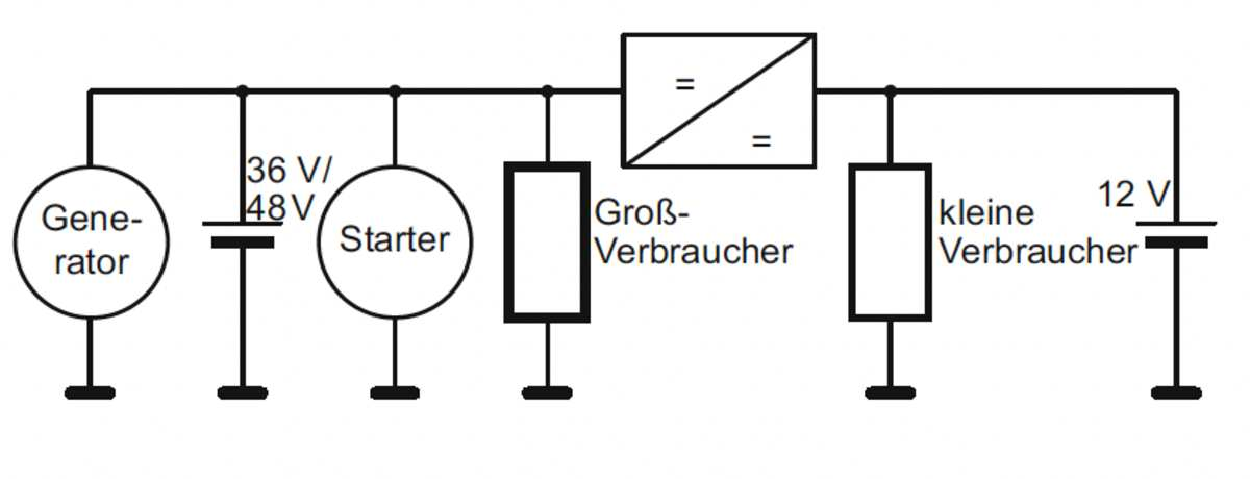
\includegraphics[width=0.7\textwidth]{images/CAN/CAN-2.pdf}
\caption{Struktur eines künftigen Mehrspannungsbordnetzes (Bild: Kai
Borgeest)}
%\label{fig:}%% anpassen
\end{figure}

Kombination aus einem 12-V-Netz für Kleinverbraucher und einem 48-V-Netz
für Großverbraucher. Beide Netze werden über einen Schaltwandler (DC/DC)
gekoppelt.

\newpage

\subsection{Energiemanagement (BMS)}\label{energiemanagement-bms}

\begin{enumerate}
\item
  Batterieüberwachung

  \begin{itemize}
  \item
    Eingriff in die Laderegelung
  \item
    Eingriff in das Motormanagement, um zum Aufladen der Batterie eine
    Mindestdrehzahl zu erzwingen.
  \item
    Ziele

    \begin{enumerate}
    \def\labelenumii{\arabic{enumii}.}
    \item
      Bestimmung des Ladezustandes (State of Charge, SOC)
    \item
      Restlebensdauer der Batterie (State of Health, SOH)
    \item
      Funktionsfähigkeit der Fahrzeugfunktionen, vor allem des Startens
      (State of Function, SOF).
    \end{enumerate}
  \end{itemize}
\item
  automatisch Verbraucher je nach Wichtigkeit und Leistungsbedarf
  abzuschalten oder auch wieder einzuschalten.
\item
  Steuerung eines hybriden Antriebssystems
\end{enumerate}

\textbf{Energiemanagement-Steuergerät / Bordnetzsteuergerät} benötigt
von der Batterie Informationen über Temperatur, Spannung und Strom.

\textbf{Batterietyp} über Diagnosetester dem Energiemanagement
mitteilen, welcher eingebaut wurde.

\textbf{Fremdstartbolzen} der bei Starthilfe anstelle des
Batterie-Minuspols zu verwenden ist, damit das Steuergerät den
Fremdstart registriert und bei seinen Berechnungen berücksichtigt.

\textbf{schweren Unfall} (Signal vom Airbag-Steuergerät) über ein Relais
das Bordnetz spannungsfrei schaltet.

Bei großen Batterien für Hybrid- und Elektrofahrzeuge werden wesentliche
Teile des Energiemanagements in die Batterie integriert.

\newpage

\section{CAN-Bus}\label{can-bus}

CAN-Bus war das erste digitale Bussystem.

\begin{figure}[!ht]% hier: !ht
\centering
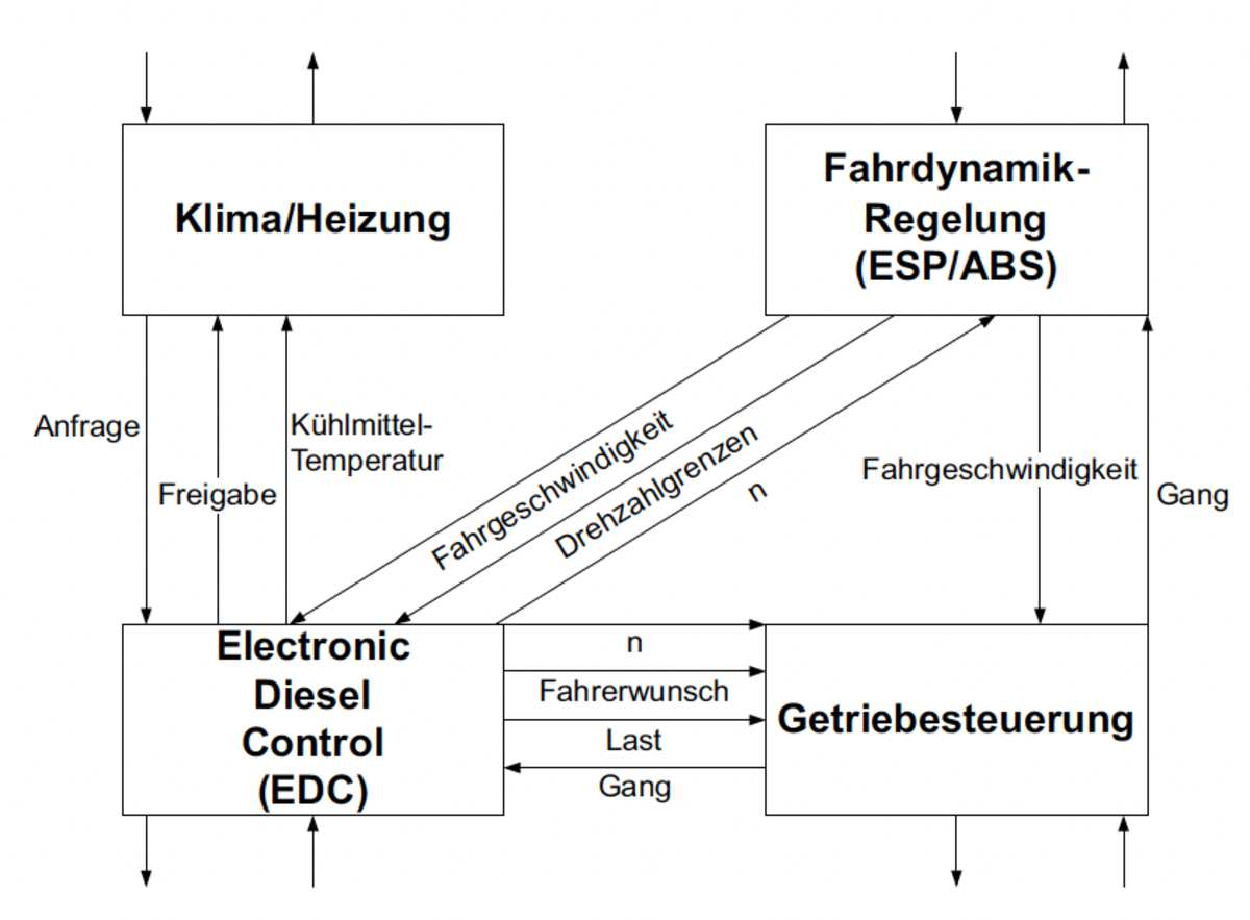
\includegraphics[width=0.7\textwidth]{images/CAN/CAN-3.pdf}
\caption{Ein kleiner Ausschnitt aus der Kommunikationsmatrix zwischen
vier Steuergeräten (Bild: Kai Borgeest)}
%\label{fig:}%% anpassen
\end{figure}

\begin{figure}[!ht]% hier: !ht
\centering
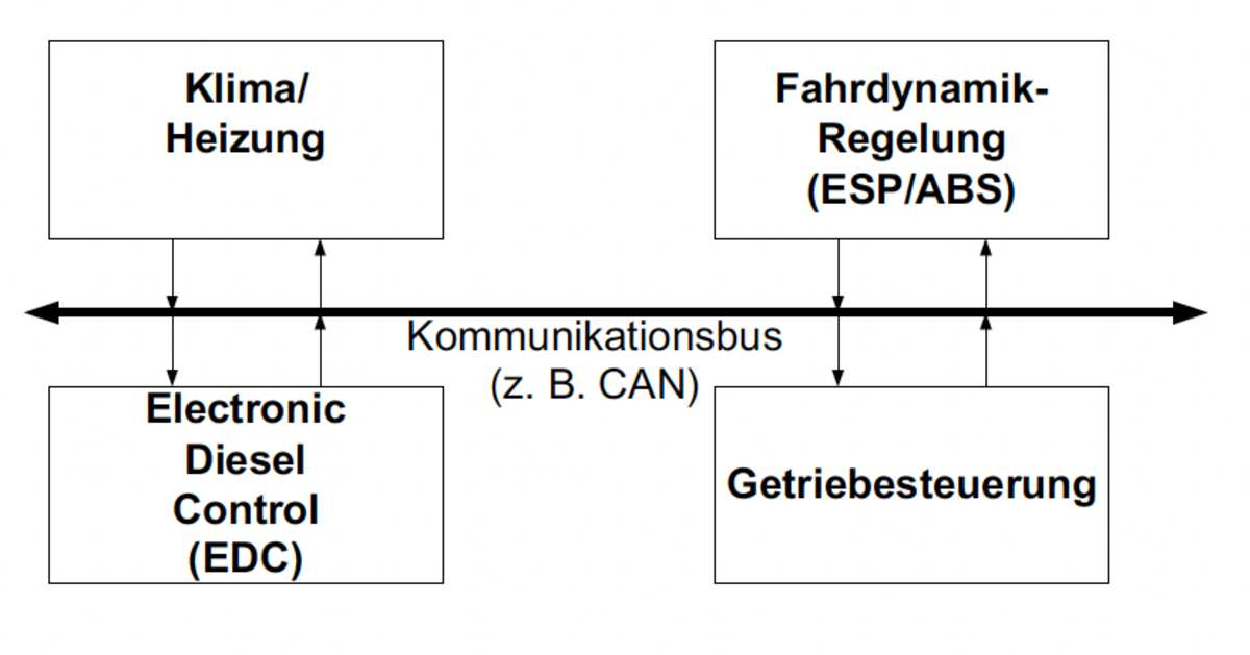
\includegraphics[width=0.7\textwidth]{images/CAN/CAN-4.pdf}
\caption{Vier über einen Bus kommunizierende Steuergeräte (Bild: Kai
Borgeest)}
%\label{fig:}%% anpassen
\end{figure}

\newpage

\textbf{Transceiver} ein Kunstwort aus Transmitter/Receiver, also
Sender/Empfänger

\begin{figure}[!ht]% hier: !ht
\centering
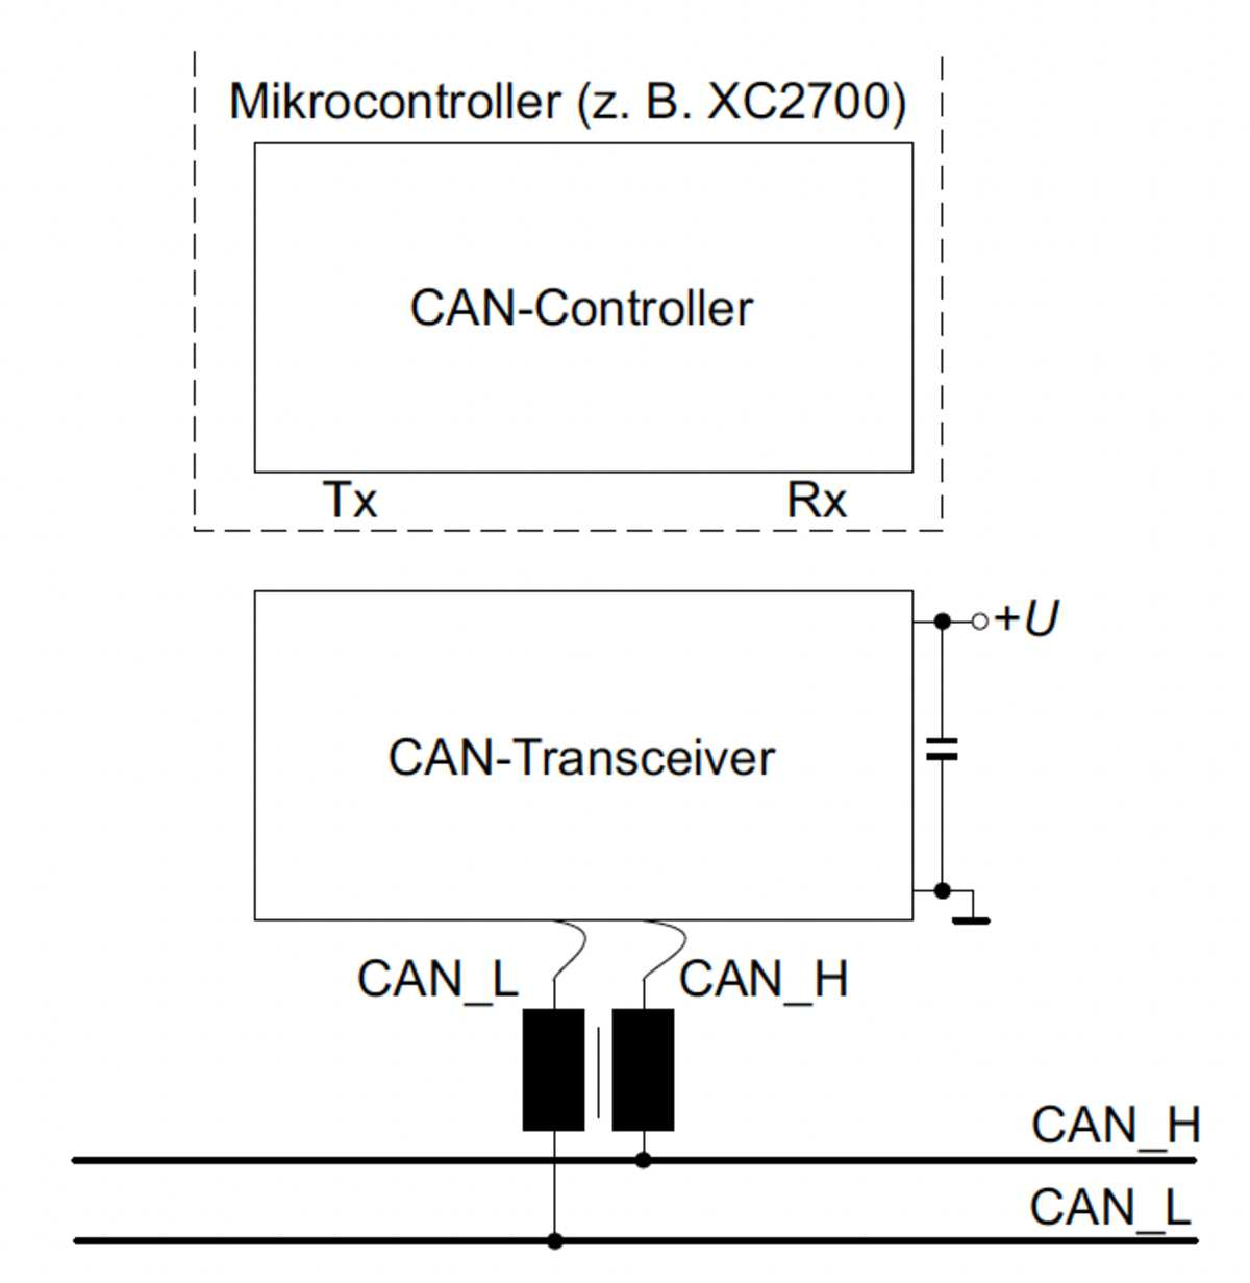
\includegraphics[width=0.5\textwidth]{images/CAN/CAN-5.pdf}
\caption{Umsetzung des OSI-Modells durch die verwendeten Bauelemente.
Der CAN-Controller erzeugt eine Nachricht mit dem gewünschten Inhalt und
sendet sie über die Leitung Tx an den Transceiver. Wenn auf dem Bus eine
Nachricht erscheint, schickt er diese über die Rx-Leitung an den
CAN-Controller, der wiederum Teil eines Mikrocontrollers sein kann, aber
nicht sein muss. Die Bezeichnungen CAN\_H und CAN\_L stehen für >>CAN
high<< und >>CAN low<<. (Bild: Kai Borgeest)}
%\label{fig:}%% anpassen
\end{figure}

\newpage

\subsection{Spannungspegel und
Störsicherheit}\label{spannungspegel-und-stoersicherheit}

Zwei verdrillte Adern stellt einen sinnvollen Kompromiss zwischen
Störfestigkeit und Kosten dar. Das Signal wird über beide Leitungen
entgegengesetzt übertragen.

\textbf{logische 1} soll gesendet werden, wird der Tx-Eingang des
Transceivers vom Controller mit einer Spannung von z. B. 5 V
angesteuert. Der untere PNP-Transistor sperrt, der obere NPN-Transistor
bekommt das invertierte Signal und sperrt ebenfalls. Der Bus behält
seine Ruhespannung von 2,5 V auf beiden Leitungen, die
Spannungsdifferenz zwischen den Busleitungen CAN\_H und CAN\_L ist 0.
Die Sendeschaltung muss nicht wie hier gezeigt mit NPN- und
PNP-Transistoren aufgebaut werden, sondern kann auch mit
Feldeffekt-Transistoren (FET) realisiert werden.

\textbf{logischen 0} leiten beide Transistoren, also wenn der Controller
das Signal am Tx-Eingang auf 0 V legt. In diesem Falle wird die Spannung
auf CAN\_H erhöht, die Spannung auf CAN\_L gesenkt.

\begin{itemize}
\item
  \textbf{CAN\_H} oder >>CAN high<< für Anhebung
\item
  \textbf{CAN\_L} oder >>CAN low<< für Absenkung
\end{itemize}

\newpage

\textbf{High-Speed-CAN}

\begin{itemize}
\item
  3,5 V auf dem CAN\_H und
\item
  1,5 V auf CAN\_L
\item
  Ruhespannung von 2,5V wird über hohe Widerstände (einige 10 -- 100
  $k\Omega$) auf beide CAN-Leitungen gelegt, damit sich die Spannung
  auf den Busleitungen beim Durchschalten der Transistoren verändern
  kann.
\end{itemize}

\begin{figure}[!ht]% hier: !ht
\centering
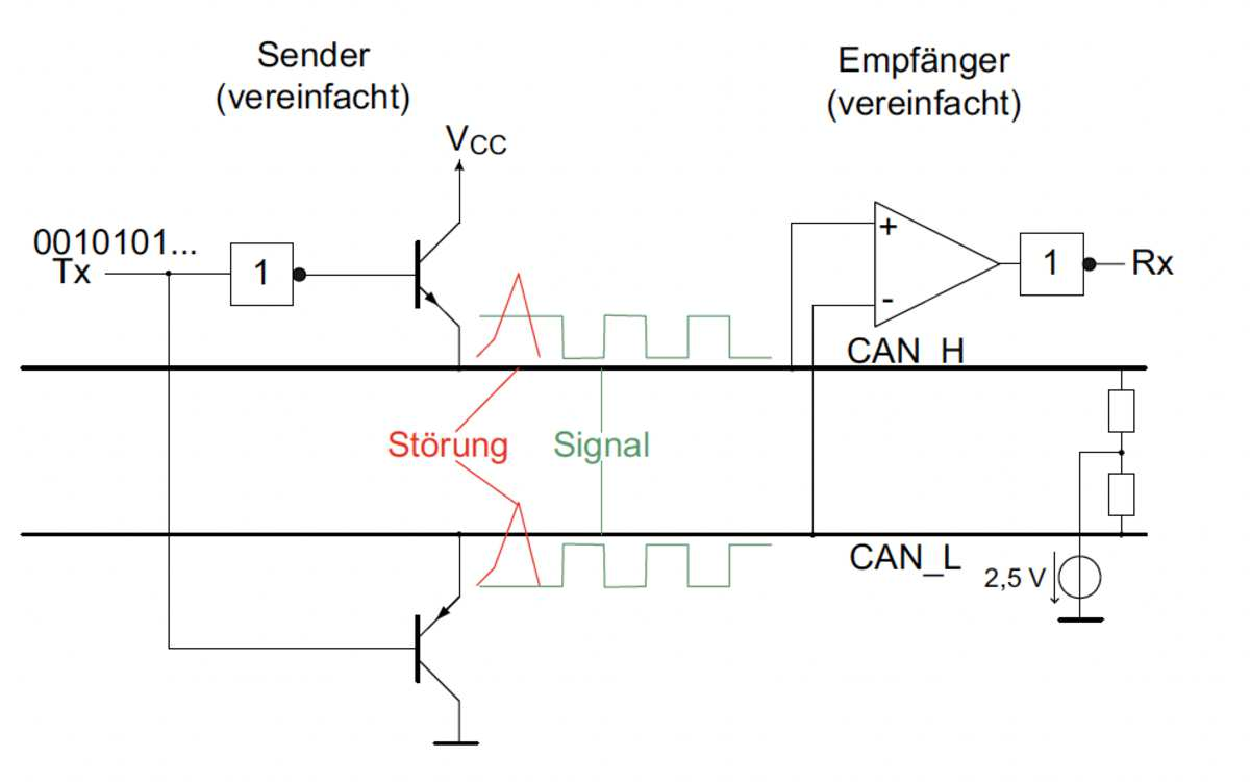
\includegraphics[width=0.5\textwidth]{images/CAN/CAN-6.pdf}
\caption{Elektrische Ansteuerung und Auswertung des CAN-Busses im
Transceiver (vereinfacht). Links ist der Sender, rechts daneben der
Empfänger eingezeichnet. Ganz rechts ist klein die Erzeugung des
Ruhepotentials von 2,5V (in vielen Highspeed-CAN-Transceivern
integriert) angedeutet (Bild: Kai Borgeest)}
%\label{fig:}%% anpassen
\end{figure}

Der Empfänger vergleicht die Spannungen auf CAN\_H und CAN\_L. Bei einer
logischen 1 liegen beide CAN-Leitungen auf 2,5 V, die Differenz ist 0.
Der nachfolgende Inverter erzeugt aus dieser 0 wieder eine 1. Bei einer
logischen 0 ist zwischen den Spannungen eine Differenz von 2 V
vorhanden. Wenn die Differenzspannung einen sicheren Minimalwert (z. B.
1 V), überschreitet, wird dies zunächst durch eine 1 signalisiert, aus
welcher der Inverter wieder die ursprüngliche 0 erzeugt.

\textbf{Low-Speed-CAN}

\begin{itemize}
\item
  Ruhespannung und rezessive Spannung

  \begin{itemize}
  \item
    5 V am CAN\_L
  \item
    0 V am CAN\_H
  \end{itemize}
\item
  dominante Spannung am

  \begin{itemize}
  \item
    1,4 V oder kleiner CAN\_L
  \item
    3,6 V oder größer am CAN\_H
  \end{itemize}
\end{itemize}

\textbf{Ist eine der beiden Leitungen defekt}, kann sie abgeschaltet
werden (Fault Tolerant CAN). Der symmetrische Betrieb wird dann
verlassen, indem die verbleibende Leitung gegen Masse betrieben wird.

\textbf{Wake-Up} (Aufwecken) Low-Speed-CAN-Transceiver können in einen
Bereitschaftszustand gehen, in dem der Sendeteil abgeschaltet ist, der
Empfangsteil aber bereit bleibt, um ein durch Kommunikation auf dem Bus
oder Aktivierung eines Pins zu ermöglichen.

\textbf{Energieeinsparung} wird ein Teilnetzbetrieb (Partial
Networking), bei dem Steuergeräte, die gerade keine Funktion erfüllen,
ihren Energieverbrauch reduzieren, immer wichtiger. Dieser benötigt ein
selektives Aufwecken einzelner Busteilnehmer.

\newpage

\subsection{Wellenwiderstand und
Abschluss}\label{wellenwiderstand-und-abschluss}

\textbf{Wellenwiderstand} sagt aus, welchen fiktiven Widerstand ein
Signal am Eingang einer Leitung >>sieht<< und damit, welchen Strom die
Quelle in die Leitung einspeist. Ist eine Kenngröße jeder Leitung, also
jedes Leiterpaares.

Wird eine Leitung nicht mit ihrem Wellenwiderstand abgeschlossen, kommt
es zu Reflexionen des Signals an ihren Enden.

\begin{enumerate}
\item
  \textbf{Leitung an den Enden offen zu lassen}

  \begin{itemize}
  \item
    kann vorkommen, wenn am Ende der Leitung sich ein Steuergerät
    befindet, dessen Transceiver einen hohen Eingangswiderstand hat (was
    durchaus üblich ist). In diesem Falle käme es zu einer Reflexion,
    das Signal würde die Leitung wieder zurücklaufen und sich mit
    anderen hinlaufenden Signalen überlagern. Damit würden andere
    Steuergeräte am Bus im schlimmsten Fall einen undefinierten
    Datenzustand empfangen, die Kommunikation auf dem Bus kann
    zusammenbrechen.
  \end{itemize}
\item
  \textbf{Leitung an den Enden kurz zuschließen}

  \begin{itemize}
  \item
    kommt nur bei Fehlern vor
  \end{itemize}
\end{enumerate}

\textbf{High-Speed-CAN} an beiden Enden mit je einem Widerstand von
nominal 120 $\Omega$ abgeschlossen, dies entspricht näherungsweise dem
Wellenwiderstand der verdrillten 2-Draht-Leitung. Um Störströme gezielt
abzuleiten, werden oft zwei Widerstände zu 60 $\Omega$ in Reihe
geschaltet und der Knoten zwischen den beiden Widerständen über einen
Kondensator von wenigen nF auf Masse gelegt.

Zweckmäßigerweise wird man diese beiden Widerstände nicht direkt in den
Kabelbaum einbauen, sondern in die an beiden Busenden sitzenden
Steuergeräte.

\textbf{Low-Speed-CAN} üblich, in jedem Knoten Widerstände jeweils gegen
Masse und Versorgungsspannung vorzusehen. Hersteller empfehlen
Gesamtabschlusswiderstände des Netzwerkes (Parallelschaltung aller
einzelnen Abschlüsse) zwischen 100 $\Omega$ und darüber. Der optimale
Abschlusswiderstand steigt also mit der Anzahl der elektrisch parallel
geschalteten Knoten im Netzwerk.

\newpage

\subsection{Verbindung von
Steuergeräten}\label{verbindung-von-steuergeraeten}

\begin{figure}[!ht]% hier: !ht
\centering
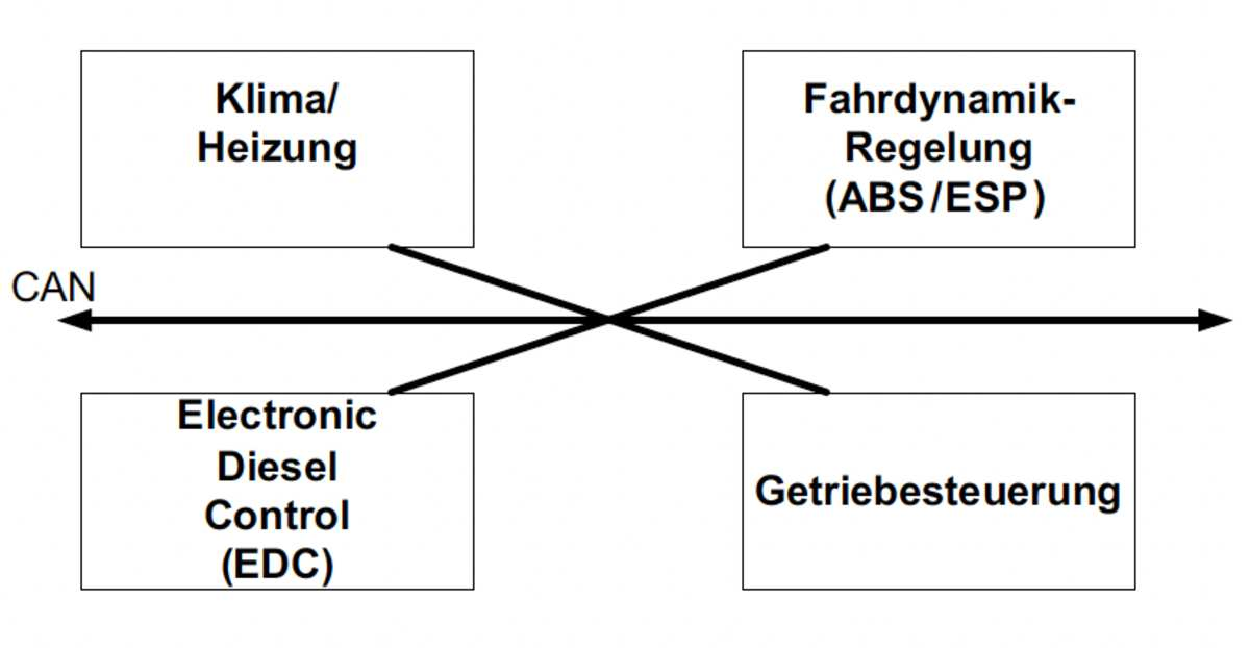
\includegraphics[width=0.5\textwidth]{images/CAN/CAN-7.pdf}
\caption{CAN-Bus mit sternförmiger Anbindung (passiver Stern) (Bild: Kai
Borgeest)}
%\label{fig:}%% anpassen
\end{figure}

\begin{enumerate}
\item
  \textbf{passive Stern}

  \begin{itemize}
  \item
    wird häufig in der Nähe des Armaturenbretts realisiert, evtl.
    existieren auch mehre Sternpunkte.
  \item
    Vorbildlich hat z. B. Audi beim A6 und beim A8 die Sternpunkte
    realisiert. Sämtliche Zugänge treffen sich an den beiden Seiten des
    Armaturenbrettes, die Verbindungen erfolgen über Brückenstecker.
  \end{itemize}
\item
  \textbf{aktiver Stern} bei dem sich ein weiteres Gerät im Sternpunkt
  befände, um jede Verzweigung mit einem eigenen Transceiver
  anzusteuern.

  \begin{itemize}
  \item
    Gateway (aktiver Stern) eines Oberklasse-Fahrzeugs mit vier
    High-Speed-Transceivern (HS) und einem Low-Speed-Transceiver (LS)
    für den langsameren Komfort-CAN. Eine CPU (Mikrocontroller) kann
    gezielt Nachrichten aufarbeiten und an andere Busse weiterleiten.
  \end{itemize}

  \begin{enumerate}
  \def\labelenumii{\arabic{enumii}.}
  \item
    High-Speed-Transceivern (HS)

    \begin{itemize}
    \item
      Antriebs-CAN
    \item
      Kombi-CAN
    \item
      ACC-CAN
    \item
      Diagnose-CAN
    \end{itemize}
  \item
    Low-Speed-Transceiver (LS)

    \begin{itemize}
    \item
      Komfort-CAN
    \end{itemize}
  \end{enumerate}
\end{enumerate}

\begin{figure}[!ht]% hier: !ht
\centering
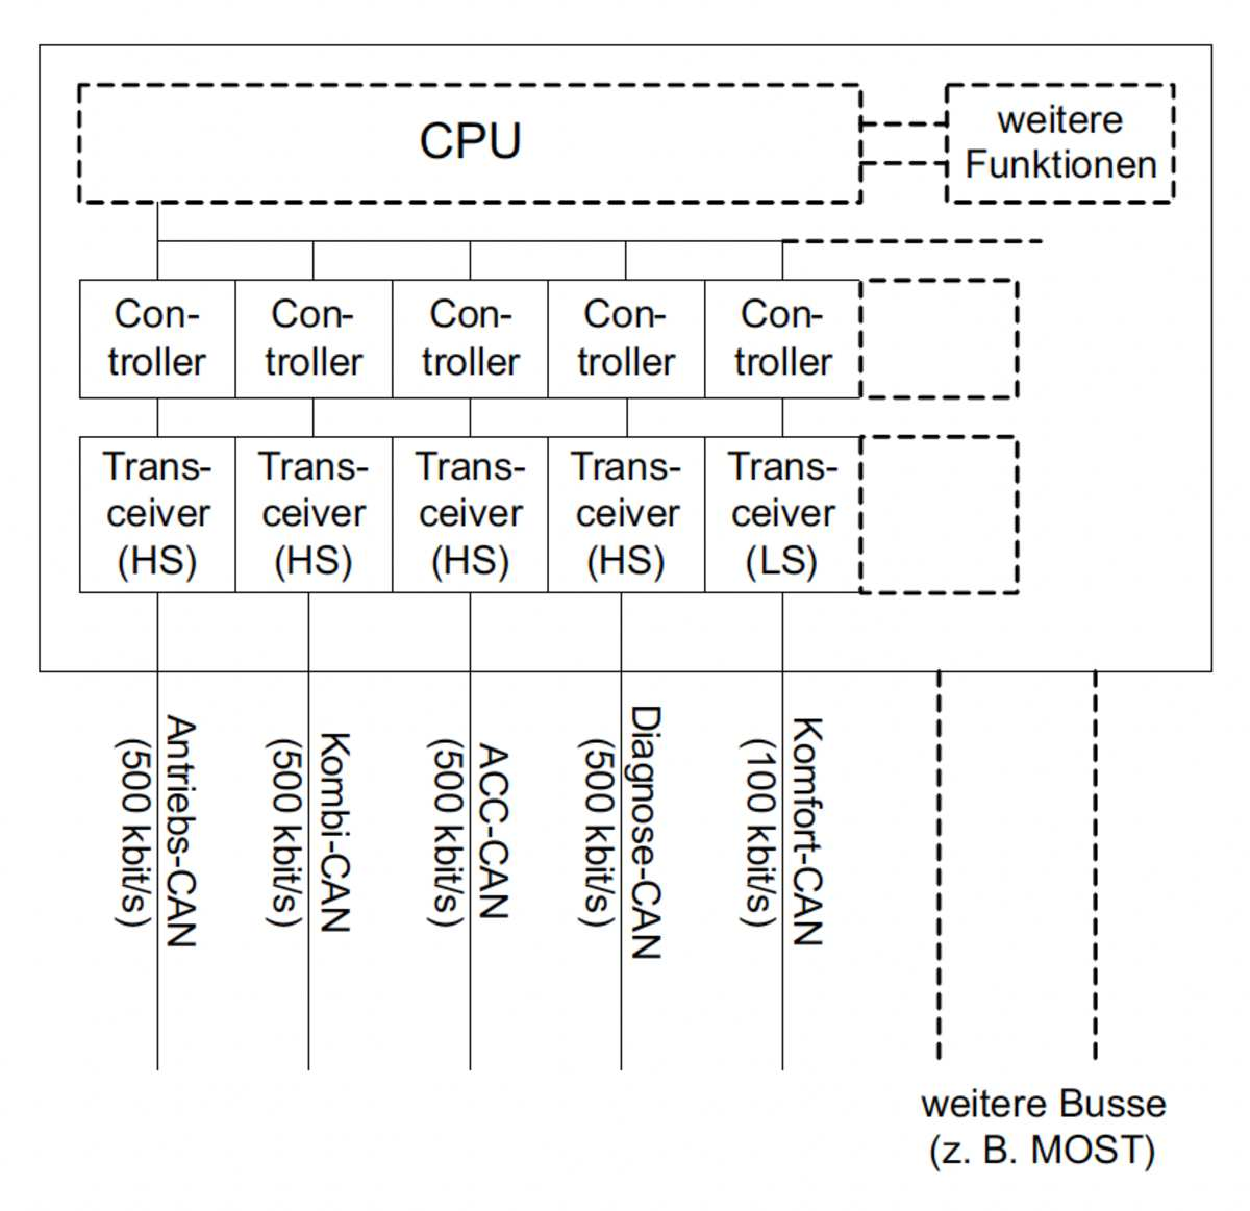
\includegraphics[width=0.5\textwidth]{images/CAN/CAN-8.pdf}
\caption{Gateway (aktiver Stern) eines Oberklasse-Fahrzeugs mit vier
High-Speed-Transceivern (HS) und einem Low-Speed-Transceiver (LS) für
den langsameren Komfort-CAN. Eine CPU (Mikrocontroller) kann gezielt
Nachrichten aufarbeiten und an andere Busse weiterleiten. (Bild: Kai
Borgeest)}
%\label{fig:}%% anpassen
\end{figure}

Inzwischen ist es üblich, in einem Fahrzeug mehrere elektrisch getrennte
CAN-Busse zu haben, die sich auch in ihren Datenraten unterscheiden
können, aber nicht müssen. Verbunden sind diese dann über einen aktiven
Sternpunkt, der auch als Gateway bezeichnet wird. Während bei Systemen
von geringer Komplexität (bis ca. 5 Steuergeräte im Fahrzeug) evtl. auf
ein Gateway verzichtet wird, besitzen Systeme von mittlerer bis hoher
Komplexität (ab ca. 50 Steuergeräte im Fahrzeug) auf jeden Fall eines.
Das Gateway kann eine zusätzliche Funktion eines möglichst zentralen
Steuergerätes, z. B. des Kombiinstruments sein, mit zunehmender
Komplexität verwendet man als Gateway ein eigenständiges Gerät, welches
nur diese Aufgabe verrichtet.
